\chapter{Background Theory and Related Work}

% THIS IS AN EXAMPLE. ALL SECTIONS BELOW ARE OPTIONAL. PLEASE CONSULT YOU ADVISOR AND DESIGN YOUR OWN SECTION

% \textthai{หัวข้อต่าง ๆ ในแต่ละบทเป็นเพียงตัวอย่างเท่านั้น หัวข้อที่จะใส่ในแต่ละบทขึ้นอยู่กับโปรเจคของนักศึกษาและอาจารย์ที่ปรึกษา}

% This is how you add the website URL: \url{http://www.cpe.kmutt.ac.th}

% Explain theory, algorithms, protocols, or existing research works and tools related to your work.

% You can cite your references like this: \cite{booch87}, or multiplie cite like this: \cite{meyer2000, atwoodmd}

\section{Introduction}
This chapter outlines the theory and related research to ensure that the development is feasible and that there are appropriate tools. Relevant knowledge will be researched and summarized, along with the technologies and programming languages to be used. Additionally, competing solutions developed by others will also be discussed in this chapter.

\section{Background}
The Business Intelligence Infrastructure team at Agoda is responsible for assisting customers in retrieving data using SQL statements. Currently, 27\% of the tickets in BI-Help are categorized as 'Query Help.' This is because customers often struggle with writing SQL statements correctly, and SQL error messages can be difficult to understand. Additionally, with multiple databases, error messages can vary, and many users deal with highly complex SQL statements. Furthermore, other teams with limited SQL knowledge also seek assistance from the BI team to retrieve data from the database. To address these challenges, the team aims to develop Query Assistance to provide an effective solution.
\section{Theory and Core Concepts}
    \subsection{Large Language Models (LLMs)}
    Large Language Models (LLMs) represent a significant advancement in artificial intelligence, engineered to comprehend and generate human-like text through comprehensive training on vast datasets. Employing sophisticated deep learning techniques, these models interpret words and sentences in context, enabling them to carry out tasks such as text generation, summarization, and sentiment analysis. Fine-tuning further refines their ability to respond accurately to specific applications, enhancing their adaptability and efficacy for targeted tasks. Additionally, with specialized training, LLMs can undertake language translation, broadening their applicability across multilingual environments. These capabilities make LLMs indispensable in modern AI solutions, addressing a wide range of language-based challenges with precision and scalability.
    \subsection{Representational state transfer application programming interface (REST API)}
    Application Programming Interface (API) is middleware that facilitates communication between two software components. Representational State Transfer (REST) is a software architectural style that defines a set of constraints and principles on how an API should behave.
    \pagebreak
    \subsection{Software Architecture Pattern}
    Software architecture plays a crucial role in software development. It is a fundamental practice for developers to create software that is high-quality, efficient, and easy to manage and maintain. Software architecture consists of patterns that have been proven over time, becoming best practices that help solve common problems in software development. By following these patterns, developers can build systems that are easier to understand, maintain, and expand.
    \cite{Arslan}

    The following outlines the importance of architectural patterns. First, software architecture acts as a visual communication tool, allowing other developers, colleagues, or even stakeholders to understand the system you are building in a much simpler way. Second, software architecture models make it easy to reuse them in other projects since you now know the decisions you made and the various trade-offs. Third, complex systems with many components and interactions need a clear structure to ensure everything works together smoothly. Fourth, systems expected to grow over time or handle high loads require careful planning to avoid bottlenecks and ensure they can scale efficiently. Fifth, long-term projects that will be developed and maintained over several years need a solid architectural foundation to prevent technical debt and ensure maintainability.
    \cite{Abbas}

    There are several architectural styles, each with unique benefits and uses. The microservices architecture is one example; it is a design methodology in which an application is constructed as a group of independent, autonomous services that communicate. Every service has a distinct purpose and functions autonomously, interacting with other services using simple protocols. The architecture of microservices has a number of important benefits. By enabling autonomous scalability of different services in response to particular demands, it guarantees effective resource allocation. Additionally, this method offers flexibility because services may be changed or removed without impacting the application as a whole. It also improves fault isolation by isolating issues within a single component, reducing the risk of systemic failures and ensuring that the failure of one service does not cause the entire system to crash. Identifying and resolving problems is often simpler in smaller, independent services. Another benefit is that teams can work on multiple services simultaneously, accelerating the development process. Incremental updates allow new service versions to be deployed gradually, minimizing downtime and ensuring smoother transitions.
    \cite{Vicki}
    \begin{figure}[H]
        \centering
        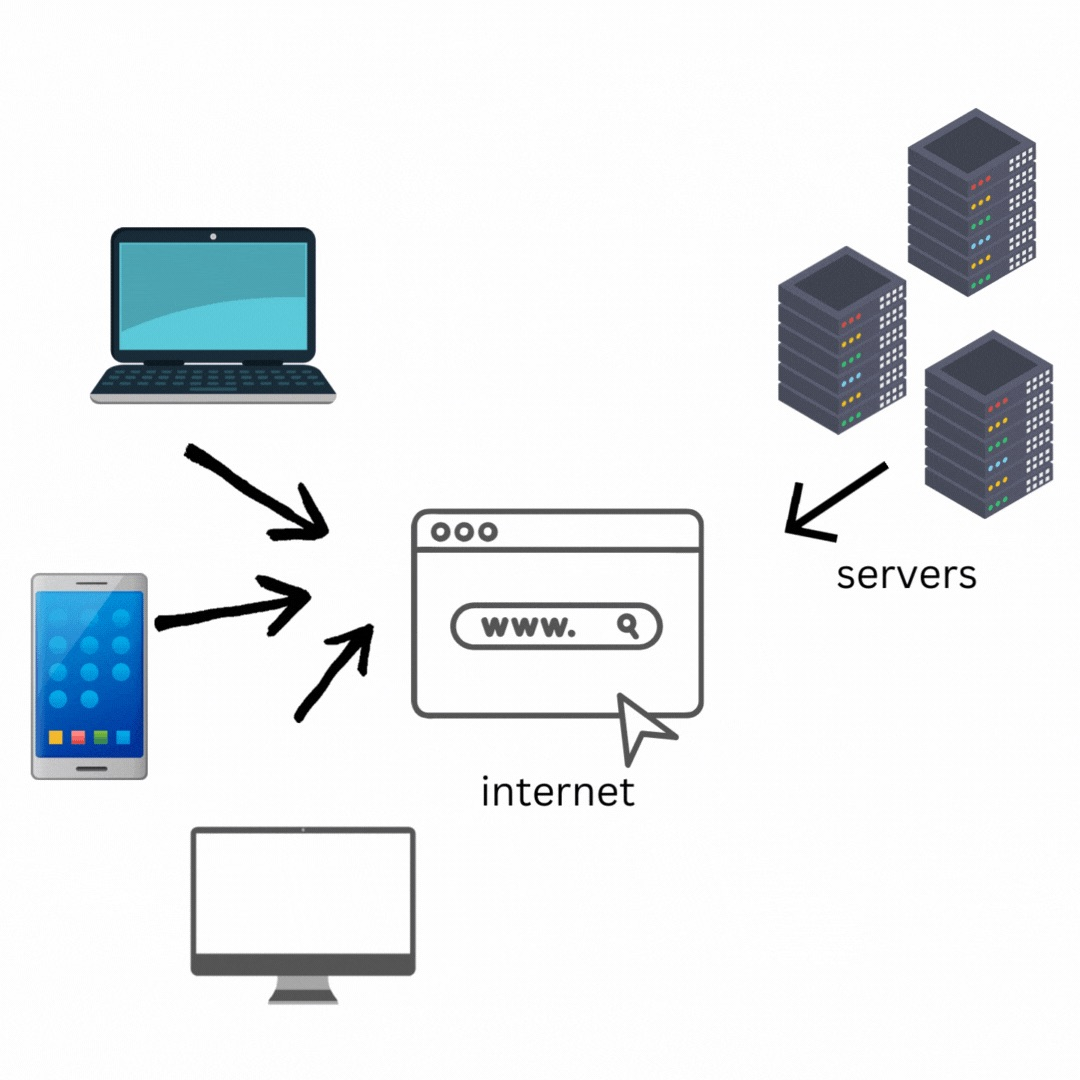
\includegraphics[width=7cm]{chapters/2/figures/eb6b7a926564d8e2d83f58f00.jpg}
        \caption[Microservices architecture]{Microservices architecture  from~\cite{Vicki}}
        \label{fig:microservices-architecture}
    \end{figure}

    The Model-View-Controller (MVC) architecture pattern is a design used to divides an application into three linked parts: the Model, View, and Controller. The Model manages the data and business logic of the application. It handles data management, upholds business rules, and reacts to queries from other parts, such the Controller and View. The View is in charge of the user interface. It sends user commands to the Controller and shows the user data from the Model. Instead of interacting directly with the Model, the View handles user inputs through the Controller.The Controller serves as a connector between the View and the Model. In order to update or retrieve data, it communicates with the Model, processes user input from the View, and takes the necessary actions.
    \cite{GeeksforGeeks}

    \subsection{Agent System}
    An agent is a software program designed to perform tasks on behalf of a user. It automates processes, makes decisions, and interacts intelligently with its environment. Agents remember knowledge from previous interactions, and use a variety of tools to modify their replies according to the situation and desired style. They are especially useful for activities that call for sequential reasoning since they may break down difficult tasks into smaller, more manageable ones. An agent needs a well-organized plan, a strong memory to monitor its progress, and the right tools to do these subtasks.

    A prompt is a crucial component of an agent's guidance since it acts as a collection of guidelines that specify the agent's response strategies, tool selection procedures, and interaction goals. It serves as a blueprint, giving the agent precise instructions so it can complete its job efficiently. By preserving a record of previous activities, an agent's memory system is crucial for handling complicated tasks. The two main forms of memory that agents use are short-term and long-term memory. Tracking ongoing interactions in short-term memory allows the agent to react appropriately to the current context. Nevertheless, this memory is only used temporarily and is deleted after the activity is finished. On the other hand, knowledge from previous interactions is stored in long-term memory. In order to make better decisions in subsequent interactions, it goes beyond mere data storage by spotting trends, learning from previous activities, and remembering relevant data. The planning strategy of an agent consists of two key stages: plan formulation and plan reflection. Agents divide a more complex work into more manageable, smaller subtasks at the plan formulation stage. Different approaches are used for work breakdown. While some strategies handle subtasks separately, others entail developing a thorough strategy in advance and carrying it out step-by-step. Some approaches break the issue down into several parts, producing ideas at each one and arranging them in a hierarchical structure, like a decision tree. The plan reflection stage serves as a feedback loop, where the agent evaluates and refines its plan to improve its effectiveness. ReAct and Reflect are two popular approaches of integrating feedback into planning. ReAct allows a large language model (LLM) to handle complicated tasks by repeating a cycle of action, observation, and cognition as needed. This approach takes into account input from the environment, which could be from other models, human input, or observations. Through the utilization of real-time feedback, ReAct enables the LLM to make dynamic adjustments to its approach, improving its capacity to address issues and deliver precise answers. Tools refers to a variety of resources that let agents interact with their surroundings in order to carry out particular activities. These duties could be coding, running queries, retrieving data from databases, or any other activity necessary for the agent to function properly. The agent uses these tools to carry out tasks, collect observations, and obtain the information required to finish subtasks and satisfy user requests by adhering to predetermined workflows.
    \cite{SuperAnnotate}
    \begin{figure}[H]
        \centering
        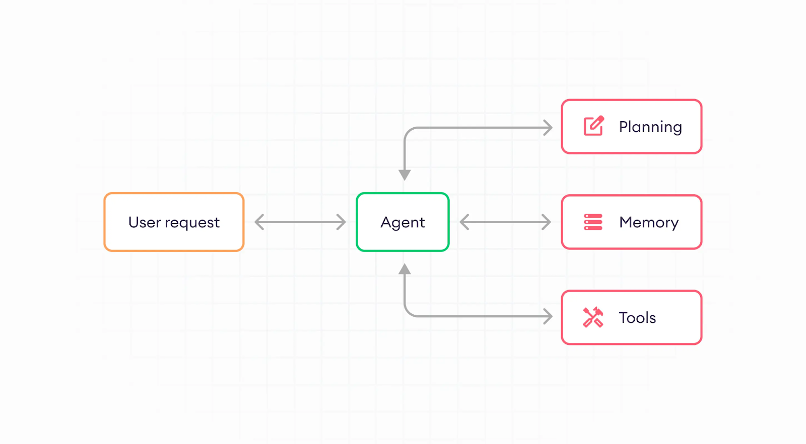
\includegraphics[width=10cm]{chapters/2/figures/agent.png}
        \caption[Agent Component]{Agent Component  from~\cite{SuperAnnotate}}
        \label{fig:agent-component}
    \end{figure}

        \subsubsection{Multi Agent System}
        A multiagent system (MAS) is composed of agents that collaborate to perform tasks to perform tasks on behalf of a user or another system. Each agent takes a unique role that it specialises in, however, all agents behave collaboratively to lead to desired result. There is a distinction between single and multiagent systems. When calling another agent as a tool, that secondary agent is part of the original agent's environmental stimuli. That information is acquired and no further cooperation takes place. Whereas multiagent systems differ by involving all agents within the environment to model each other's goals, memory and plan of action. Multiagent systems can operate under many architectures. For example, network structure is a structure where each agent can communicate with every other agent and it can make its own decision which other agent to call next. Supervisor structure is different because every agent need to communicates with a single supervisor agent after it done. Supervisor agent makes decisions on which agent should be called next. Hierarchical is a generalization of the supervisor architecture and allows for more complex control flows. Lastly Custom multi-agent structure, each agent communicates with only a subset of agents. Parts of the flow are deterministic, and only some agents can decide which other agents to call next.
        \cite{Gutowska} \cite{LangGraph}
        \begin{figure}[H]
            \centering
            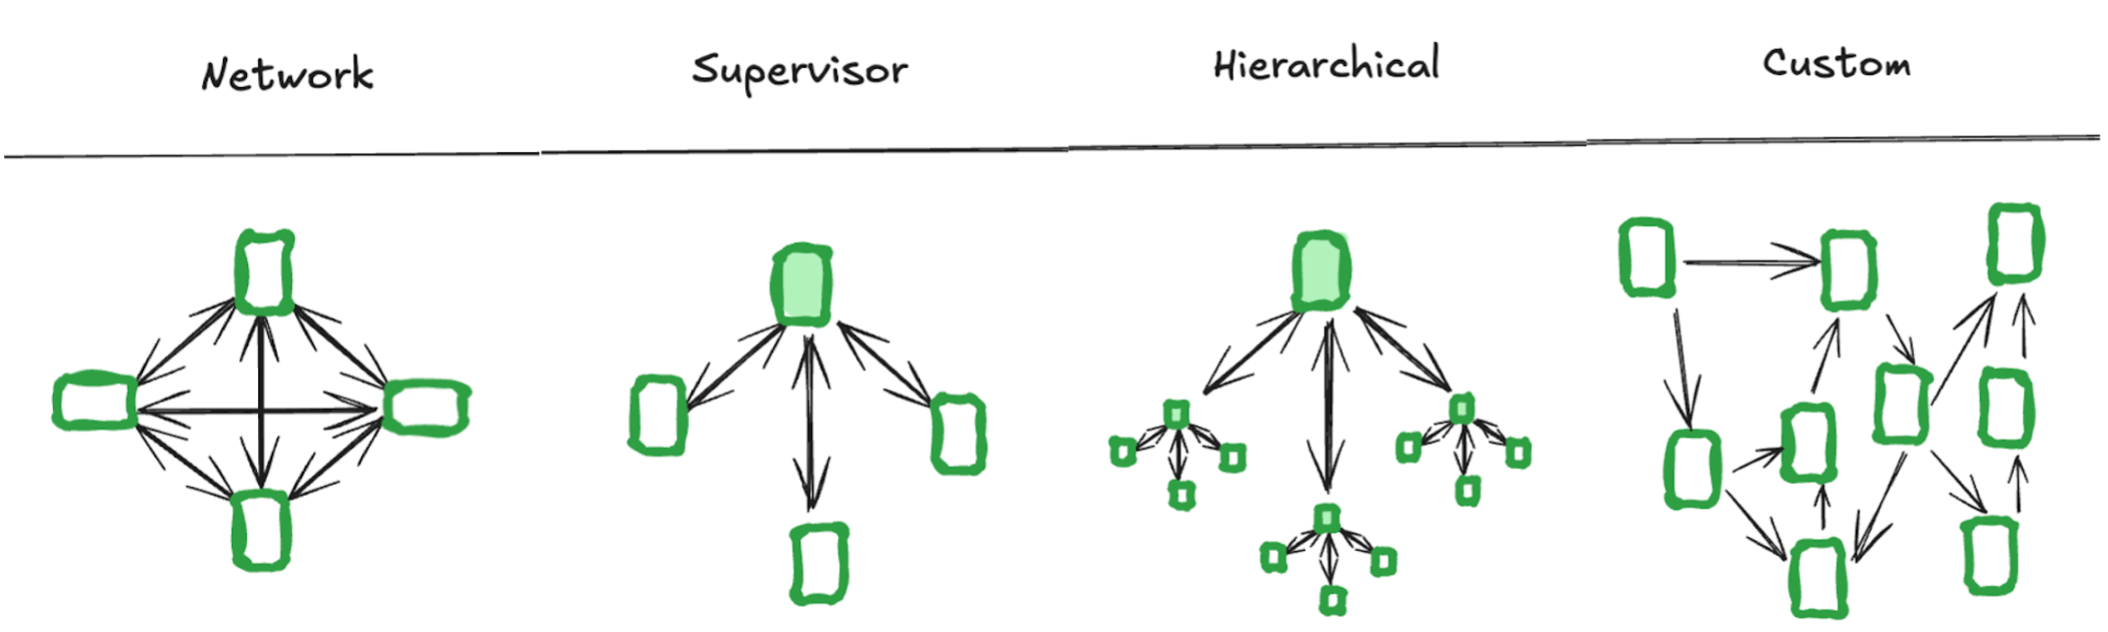
\includegraphics[width=10cm]{chapters/2/figures/multi-agent.png}
            \caption[Multi-Agent Structure]{Multi-Agent Structure  from~\cite{LangGraph}}
            \label{fig:multi-agent}
        \end{figure}

        Even though individual agents are very powerful on their own—they can use tools, establish subtasks, and learn from interactions—multi-agent systems frequently perform better than single-agent systems because they can share resources, automate tasks, and optimize processes. Multi-agent systems enable the sharing of learned experiences, greatly increasing time efficiency and overall performance, as opposed to several agents independently learning the same policies Multi-agent systems offer several advantages over single-agent systems by leveraging collaboration and resource sharing. They increase accuracy by decreasing hallucinations since agents can verify one other's work to reduce mistakes and increase dependability. Additionally, by distributing duties among agents, these systems are better able to manage broader contexts and enable them to work together to analyze more information. Multi-agent systems further increase efficiency by allowing agents to execute numerous tasks at once through parallel processing, which speeds up reaction times and boosts output. Finally, they are perfect for tackling complicated problems because of their collaborative capabilities, which allow them to integrate the skills and competencies of various agents and promote creativity in areas like strategic planning and scientific research.
        \cite{SuperAnnotate2}

    \subsection{Retrieval-augmented generation (RAG)}
    Retrieval-Augmented Generation (RAG) is a natural language processing (NLP) technique that enhances the quality of generated text by combining retrieval-based and generation-based methods.
    \cite{Martineau}
        \begin{itemize}
        \item  Retrieval: The system searches a large database to find relevant information related to the input query, ensuring access to accurate and up-to-date data.
        \item  Augmentation: The retrieved information is then combined with the original query to enhance or extend it.
        \item  Generation: Using a text generation model (such as GPT-3), the system produces a coherent and informative response based on the augmented input (original query + retrieved information)
        \end{itemize}

    \subsection{Fine-tuning}
    Fine-tuning is the process of adapting a pretrained machine learning model to perform better on a specific task by continuing its training on a targeted dataset. Rather than training from scratch, fine-tuning leverages a pretrained model’s existing knowledge while refining it to improve performance in a specialized domain. This process is especially useful when the pretrained model is highly capable in general tasks but lacks precision in particular applications.

    Fine-tuning involves adjusting the model's weights through additional training on domain-specific data, allowing it to retain general language understanding while enhancing its ability to generate accurate and relevant outputs for the desired task. Depending on the level of adaptation required, fine-tuning can be performed at different levels, such as full-model fine-tuning, where all parameters are updated, or more efficient approaches like Low-Rank Adaptation (LoRA) and adapter layers, which modify only a subset of the model while keeping most of it frozen.

    A crucial component of fine-tuning is the dataset selection and preprocessing. High-quality, task-specific datasets improve the model’s ability to generalize within the domain while minimizing biases. Overfitting, where the model memorizes training data rather than learning underlying patterns, is a key challenge that must be mitigated through regularization techniques and careful hyperparameter tuning.

    Fine-tuning is widely used in applications requiring specialized knowledge, such as SQL generation and modification, legal and medical document processing, and sentiment analysis. It allows Large Language Models (LLMs) to surpass their default capabilities, making them more efficient in handling structured queries, domain-specific terminology, and context-sensitive tasks.

    The refinement process in fine-tuning also includes periodic evaluation and iteration, ensuring that the model not only improves in accuracy but also maintains its ability to generalize to unseen data. By systematically modifying a pretrained model through domain adaptation, fine-tuning serves as a powerful technique for achieving optimal performance in specialized machine learning tasks.
    \cite{levcraigfinetuning}

\section{Languages and technologies}
    \subsection{Python}
    Python is a high-level programming language that serves multiple aspects of software development. Python offers a wide array of libraries that are invaluable for various tasks. For this project, we focus on utilizing Python to develop Large Language Models (LLMs).
    \subsection{LangChain}
    LangChain is a framework designed for building applications using Large Language Models. It streamlines the development process by enabling seamless transformation and integration of information through interconnected components.
    \subsection{LangChain Community}
    LangChain Community is a third-party integrations library designed to work alongside LangChain, enabling seamless interaction with various external tools, APIs, and frameworks. It extends the core functionalities of LangChain by providing pre-built integrations with databases, vector stores, LLM providers, and other essential components for AI applications.
    \subsection{Flask}
    Flask is a micro web framework for Python designed to enable the creation of lightweight and scalable web services. It offers simplicity and flexibility, making it an excellent choice for both small-scale applications and complex web services.
    \subsection{SQLAlchemy}
    SQLAlchemy is an SQL toolkit and Object Relational Mapper (ORM) for Python that assists in creating and managing relational databases. It provides a concise and efficient way to access and manipulate database data.
    \subsection{Alembic}
    Alembic is a lightweight database migration tool designed for use with SQLAlchemy. It helps ensure versioned consistency of the database schema by applying incremental changes in a controlled manner based on initial configuration settings.
    \subsection{Docker}
    Docker is a Container as a Service (CaaS) platform that is used to create isolated environments for running applications and storing data. It addresses hardware limitations and ensures consistent deployment across different environments.
    \subsection{GitLab CI}
    GitLab CI is a tool used for automation that works in coordination with GitLab to automate tasks such as testing, building, and deployment.
    \subsection{MLflow}
    MLflow offers a centralized platform for model building, deployment, and maintenance, streamlining the intricate ML lifecycle.  In addition to encouraging cooperation and guaranteeing that ML projects are solid, transparent, and prepared for real-world difficulties, it simplifies logging, organizing, and lineage. MLflow simplifies the ML workflow, supporting practitioners through all stages of development and deployment with a wide range of features and libraries.
    \cite{mlflow}
        \subsubsection{MLflow Tracking}
        The MLflow Tracking is a user interface and API that allows you to log metrics, output files, code versions, and parameters while your machine learning code is executing and to view the results afterward. MLflow supports LangChain integration through MLflow Tracing, Fluent APIs, or lower-level Client APIs, enabling trace data recording for future review, debugging, and analysis.
        \begin{figure}[H]
            \centering
            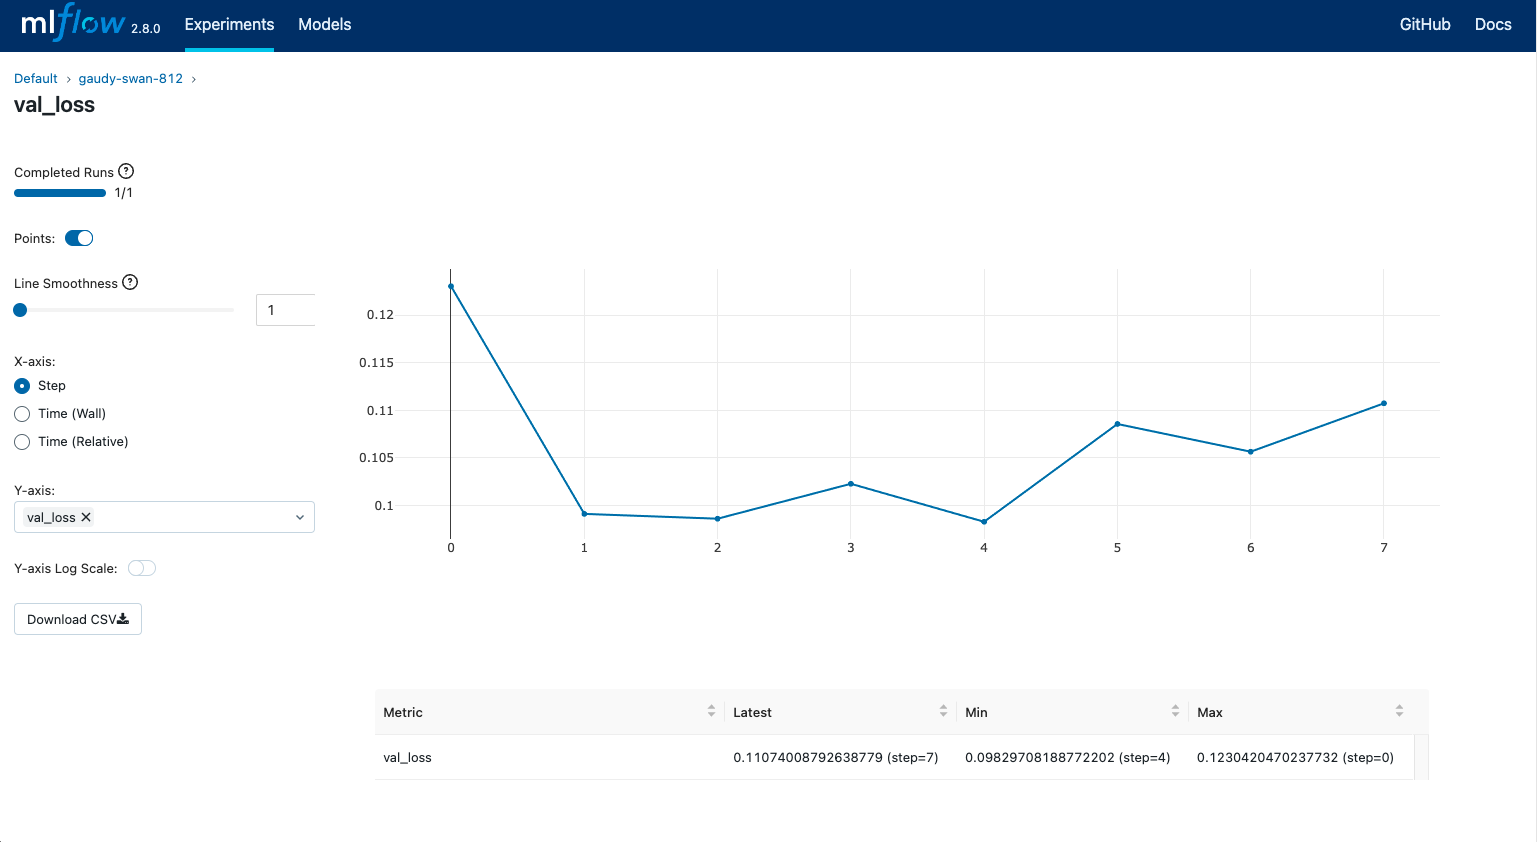
\includegraphics[width=10cm]{chapters/2/figures/mlflow-tracking-metrics-ui.png}
            \caption[MLflow Tracking]{MLflow Tracking  from~\cite{mlflow}}
            \label{fig:mlflow-tracking-metrics-ui}
        \end{figure}
        \subsubsection{MLflow Model Registry}
        Model Registry helps with version control for ML models. It manages different model versions, tracks their status, and ensures smooth deployment. It provides a centralized platform with tools and an interface to manage an MLflow Model's lifecycle, including tracking its history, versions, aliases, tags, and annotations.
        \subsubsection{MLflow Deployments for LLMs}
        The MLflow AI Gateway facilitates the usage and management of large language models (LLMs), such as Anthropic and OpenAI.  In addition to securely storing API keys in one location, it offers a single access point for managing LLM requests, lowering the possibility of their exposure.  With only a change to the gateway's settings, you may add additional LLM providers or kinds without having to modify your apps.  Because of this, it's an excellent solution for businesses that frequently employ LLMs and want a safe and easy way to handle them.
\pagebreak
        \subsubsection{Model Evaluation}
        The Model Evaluation is designed for detailed model analysis, enabling objective comparisons between traditional ML algorithms and advanced LLMs. It assesses model performance on chosen datasets, supports tasks like classification, regression, and LLM tasks (e.g., text summarization, classification, and generation), computes metrics, generates performance plots, provides model explanations, and logs results to MLflow Tracking. It also allows adding custom metrics and artifacts for deeper analysis, including creating custom metrics that can be evaluated using the Model URI of an OpenAI, Gateway, or Deployments judge model.
        \subsubsection{Prompt Engineering UI}
        This user interface-focused element offers a specialized fast engineering environment that facilitates rapid experimentation, improvement, assessment, testing, and deployment.
        \begin{figure}[H]
            \centering
            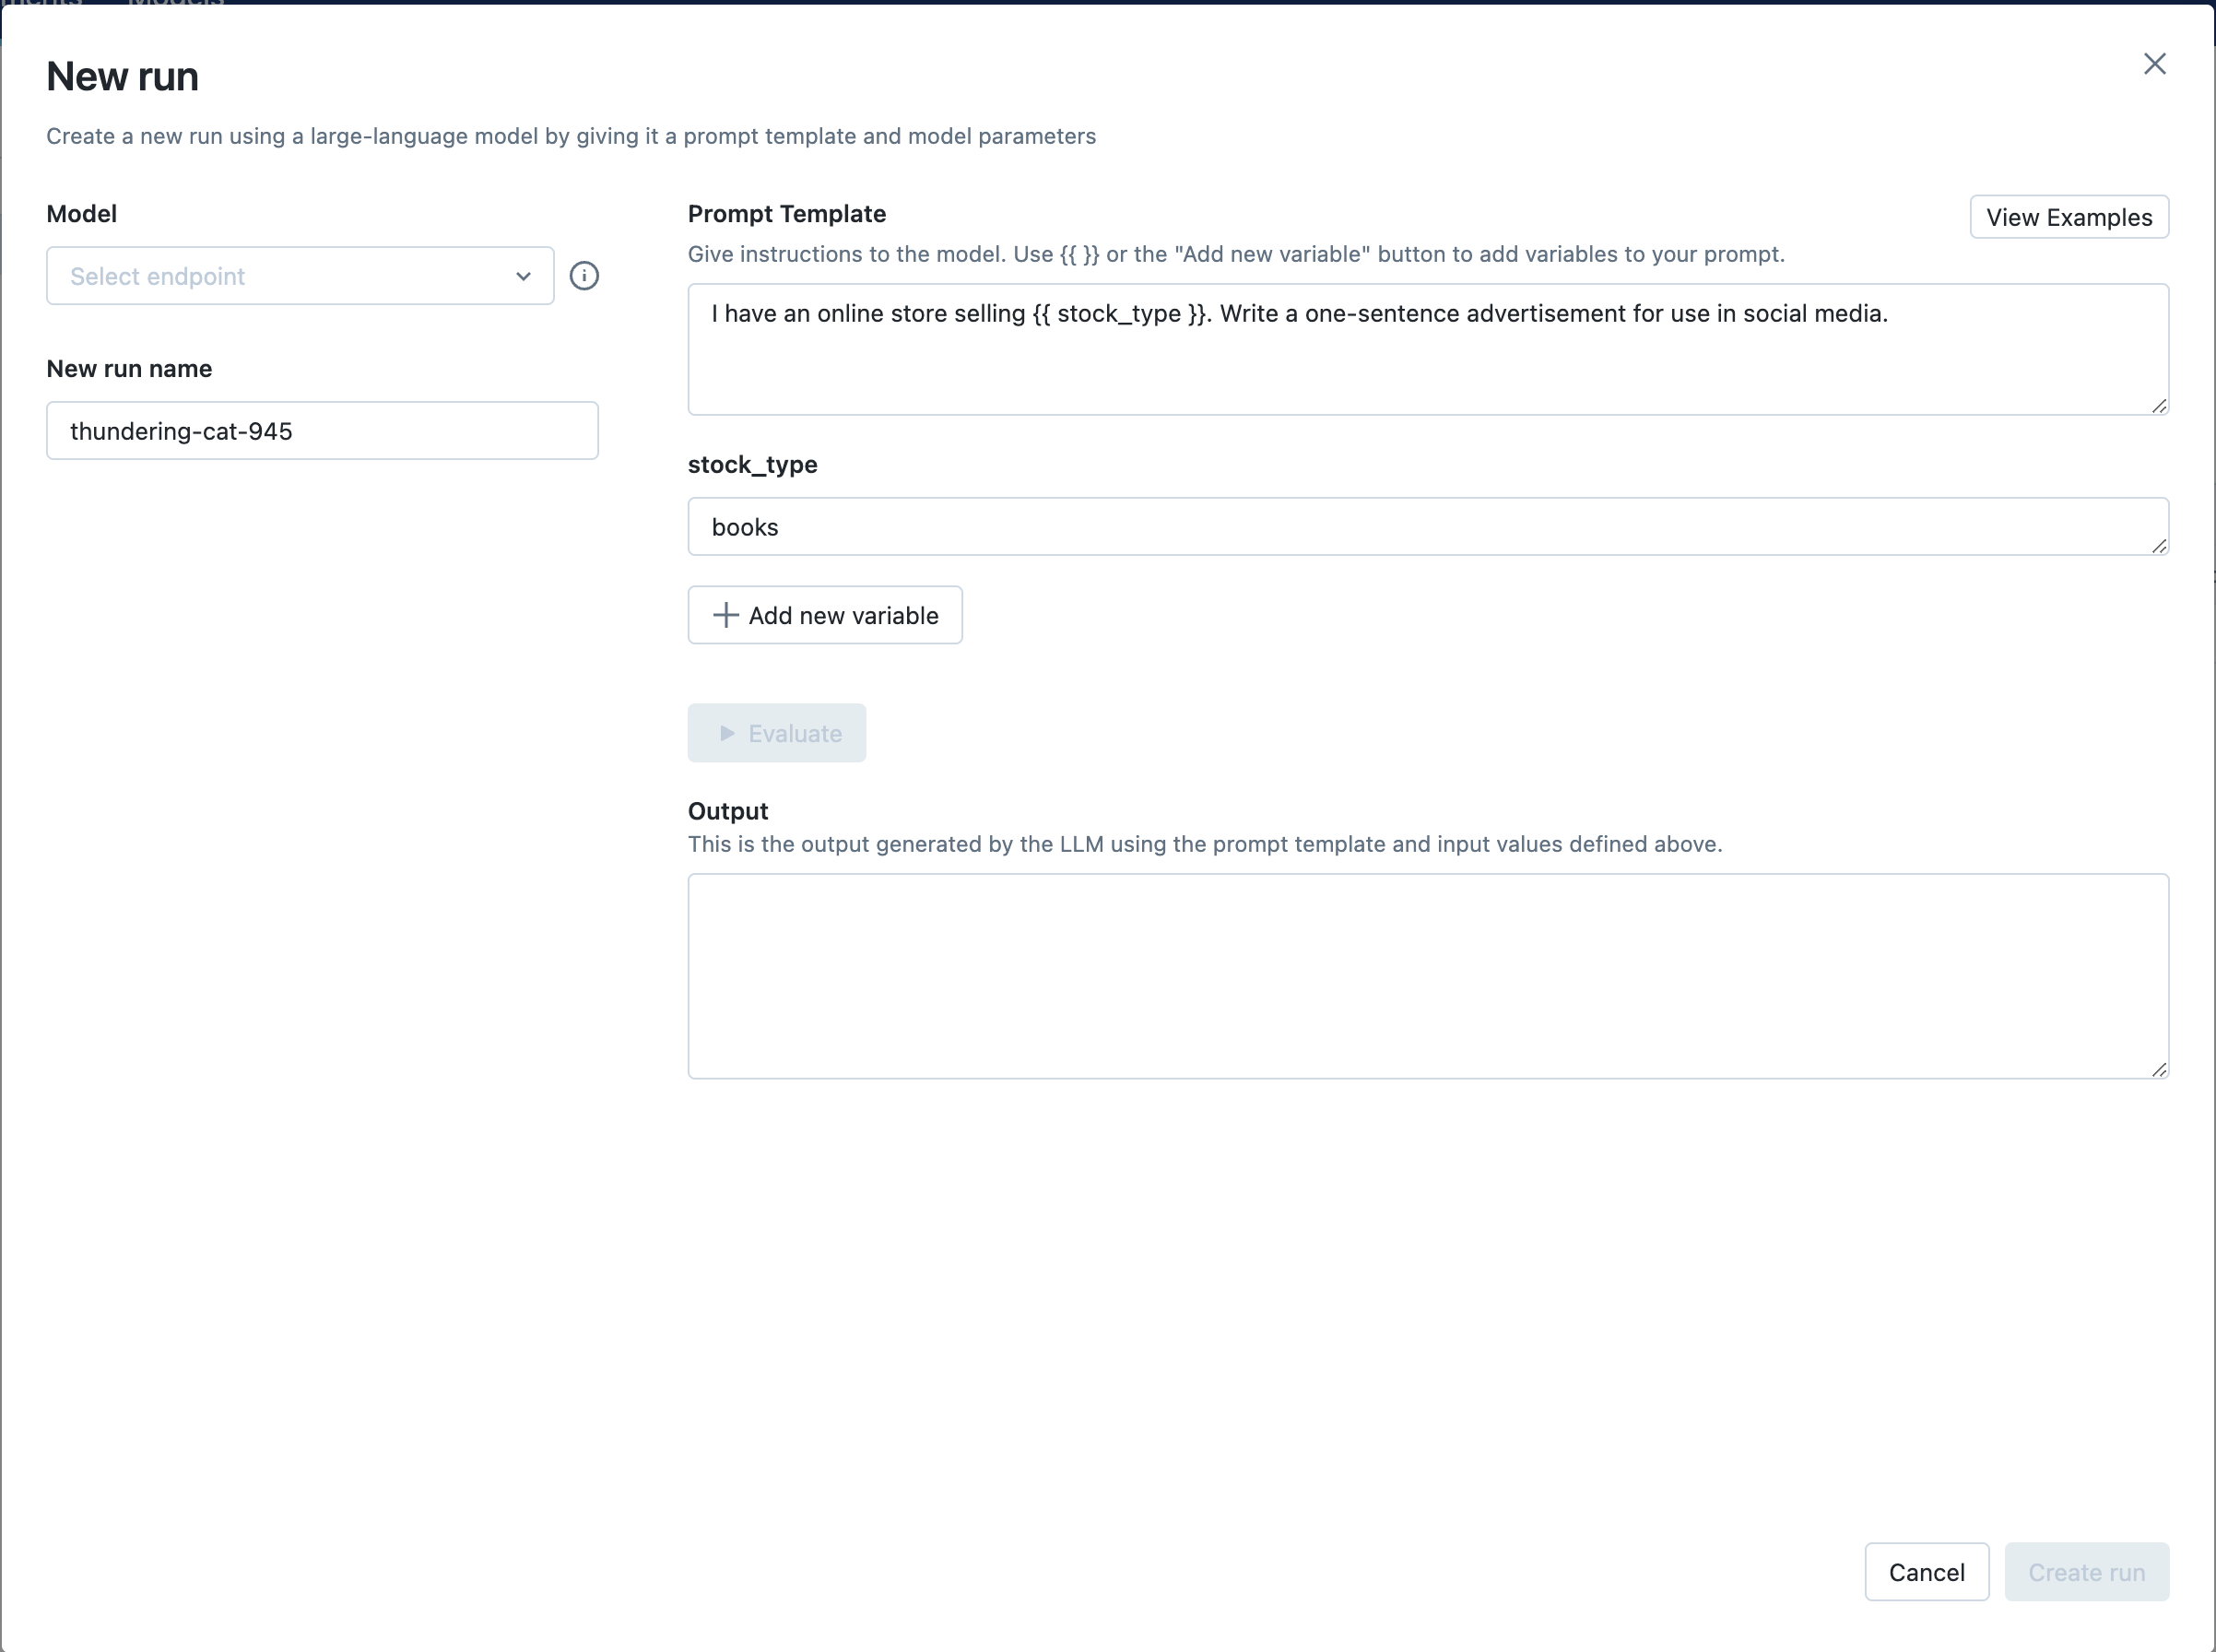
\includegraphics[width=10cm]{chapters/2/figures/prompt_modal_1-51ecbda29dcb90d4b7ed59a996470b87.png}
            \caption[Prompt Engineering UI]{Prompt Engineering UI  from~\cite{mlflow}}
            \label{fig:mlflow-prompt-engineering-ui}
        \end{figure}
        \subsection{MLflow Projects}
        An MLflow Project provides a standardized format for packaging data science code to ensure reusability and reproducibility. It relies on conventions and includes an API and command-line tools, enabling projects to be executed and linked together into workflows.

\pagebreak
\section{Database}
    \subsection{PostgreSQL}
    PostgreSQL is an open-source object-relational database management system (ORDBMS) with a robust set of features that support development, including advanced security and custom data types. In this project, we focus on leveraging PostgreSQL's capabilities to create new data types for storing vector variables.
    \subsection{Impala}
    Impala is a high-speed SQL query engine built to process large datasets stored in Hadoop clusters. Written in C++ and Java, it is open-source and delivers better performance and lower latency than other SQL engines for Hadoop. By combining the SQL features of traditional databases with the scalability of Hadoop, Impala provides a database-like experience for users. It enables fast access to data in the Hadoop Distributed File System (HDFS) and works seamlessly with components like HDFS, HBase, Metastore, YARN, and Sentry.
    \cite{Tutorialspoint}
    \subsection{Vertica}
    Vertica is an MPP (massive parallel processing) data warehouse platform specifically designed to handle big data, making it a great choice for managing large datasets that traditional databases cannot efficiently process. Its seamless integration with Hadoop makes it highly suitable for advanced data analytics workflows. Vertica is also a cost-effective solution, offering flexibility and scalability as a self-managed database. It can be deployed on commodity hardware, allowing users to start with a smaller setup and expand their data warehouse as their needs grow. Furthermore, Vertica's columnar storage ensures exceptional performance, delivering high speed and efficiency. Unlike many other data storage platforms, it eliminates the need for indexes or materialized views, making it a faster and more efficient option
    \cite{Tobin}
\pagebreak
    \subsection{StarRocks}
    StarRocks is a high-performance, next-generation analytical data warehouse made for multi-dimensional, real-time, and highly concurrent data analysis. A completely vectorized execution engine, a columnar storage engine with real-time updates, and sophisticated features like a cost-based optimizer (CBO) and intelligent materialized views are all part of its MPP (massively parallel processing) design. Real-time and batch data intake from several sources is supported by StarRocks, which also makes it possible to analyze data directly in data lakes without the need for migration.  It is highly scalable, reliable, and easy to maintain, making it ideal for OLAP scenarios like real-time analytics, ad-hoc queries, and data lake analytics. By leveraging the MPP framework, StarRocks splits query requests into parallel tasks across multiple machines, fully utilizing CPU and memory resources to deliver exceptional performance that scales with the cluster size.
    \cite{StarRocks}
    \subsection{Spark}
    Apache Spark is an open-source, distributed processing system designed for big data workloads, offering in-memory caching and optimized query execution for fast analytics on data of any size. It allows code reuse for a variety of workloads, including batch processing, real-time analytics, machine learning, and graph processing, and it supports development in Java, Scala, Python, and R. Spark's essential qualities have led to its widespread adoption across industries by companies such as FINRA, Yelp, and Zillow. They include flexibility in supporting numerous programming languages, in-memory computing that speeds up analytics by storing data in RAM, and fast processing with its Resilient Distributed Dataset (RDD), which makes it 10 to 100 times quicker than Hadoop. Additionally, Spark excels in real-time processing, handling streaming data for instant results, and offers advanced analytics tools like SQL queries and machine learning algorithms, making it a powerful solution for comprehensive data analysis
    \cite{Joseph}
    \subsection{Microsoft SQL}
    Microsoft SQL Server is a relational database system with a Database Engine for data storage, access, processing, and security. Beneath it, SQLOS manages memory, I/O, job scheduling, and data locking. Above, a network layer uses the Tabular Data Stream protocol for communication. At the user level, T-SQL is used for data management, database creation, security, and backups. Microsoft SQL Server suits mid-to-large organizations prioritizing scalability, security, Microsoft integration, and robust data tools, with the budget for licensing. However, it may not fit those needing easy customization, open-source reliance, non-Windows platforms, tight budgets, niche performance, or avoiding vendor lock-in.

    Microsoft SQL Server is scalable for any organization size, offers strong security features, integrates well with Microsoft tools, and includes data analysis tools like Reporting and Analysis Services. It supports multiple programming languages, handles large data volumes, provides automatic backups, and connects easily to cloud platforms like Azure. With flexible pricing and a large user community, it is ideal for big projects and seamless data management. However, Microsoft SQL Server has drawbacks like high costs, complexity in setup and management, resource intensity, and limited platform support beyond Windows. Licensing can be confusing, and performance may lag in specific scenarios. Customization often requires extra development, and integration with open-source tools is limited, potentially leading to vendor lock-in.
    \cite{XTIVIA}


\section{Related research / Competing solutions}
    \subsection{SQLAI.ai}
    SQLAI.ai is a tool designed to assist with both SQL and NoSQL databases. It helps beginners learn SQL and allows SQL users to enhance their skills, accelerate their workflow, and optimize their queries. The tool was developed by a fast-moving startup based in Berlin, Germany. SQLAI.ai uses GPT-4, which they describe as the world's leading AI model. They emphasize that they always use the latest and most powerful AI model available to ensure the highest quality results. There are seven features in this tool that assist users with both SQL and NoSQL, namely: generate SQL query, optimize SQL queries, fix SQL queries, explain SQL queries, simplify SQL query, format SQL query, and analyze your data. The tool supports 23 databases, including well-known ones such as MySQL, PostgreSQL, SQL Server (MS), Oracle PL/SQL, BigQuery, SQL, MariaDB, SQLite, MongoDB, DynamoDB, OrientDB, GraphQL, and Vertica. There are three ways users can obtain the database schema: by adding it manually with files, using AI to classify the file format and handle it automatically, or by connecting directly to the database. In terms of security, the tool limits the storage of sensitive data, e.g., it never stores actual database content. It only stores database schema (table and column names and data types) and credentials, which are fully encrypted. The actual database content is never stored. Users can then choose the services they want to use.
    \cite{SQLAI}

    There are three functions that both SQLAI.ai and Query Assistance share: generate SQL query, optimize SQL queries, and fix SQL queries. For fixing and optimizing SQL queries, SQLAI.ai provides more freedom for the user by offering a list of tailored fix suggestions for the SQL query. Users can choose the one they want to apply, and the AI will instantly generate a corrected query reflecting the applied step. Moreover, users can undo steps and view the differences between the original SQL query and the current one. On the other hand, Query Assist automatically fixes the SQL query and outputs only the corrected SQL query with some explanation. For generating SQL queries, both tools have similar features, but SQLAI.ai allows users to further adjust the query. Additionally, SQLAI.ai has an interface that, if the user is connected to a database, allows them to run queries directly by clicking the run button, displaying the results in a table, and generating an AI-created chart.
    \cite{SQLAI}
    \begin{figure}[H]
        \centering
        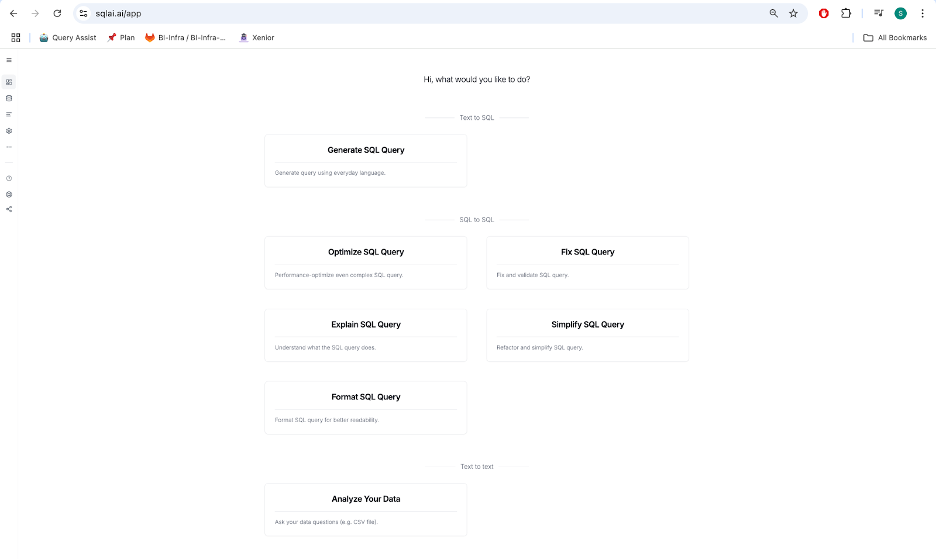
\includegraphics[width=10cm]{chapters/2/figures/sqlai.png}
        \caption[SQLAI.ai features]{SQLAI.ai features  from~\cite{SQLAI}}
        \label{fig:sqlai}
    \end{figure}

    \subsection{QueryGPT}
    Uber processes millions of interactive queries every month. Since these queries must be manually created in the editor and include exploring the data dictionary for relevant data, writing them usually takes ten minutes. QueryGPT automates the creation of queries, cutting down on time to just three minutes while ensuring accuracy. Teams will be able to save time and effort as a result of this substantial productivity improvement. By automating tedious operations, QueryGPT frees up staff members to concentrate on more valuable work, which eventually boosts organizational efficiency.

    QueryGPT was first introduced as a proposal during Uber's Generative AI Hackdays, where the idea was first conceptualized. Since then, the project has undergone continuous development and refinement, evolving from a simple concept into a production-ready service. The system not only generates SQL queries but also provides an explanation from the LLM on how the query was created, as shown in Figure 2.6, offering transparency and clarity to users. This combination of automation and explanation has made QueryGPT a valuable tool for improving query generation efficiency at Uber. The QueryGPT use OpenAI GPT-4 Turbo
    \cite{QueryGPT}
    \begin{figure}[H]
        \centering
        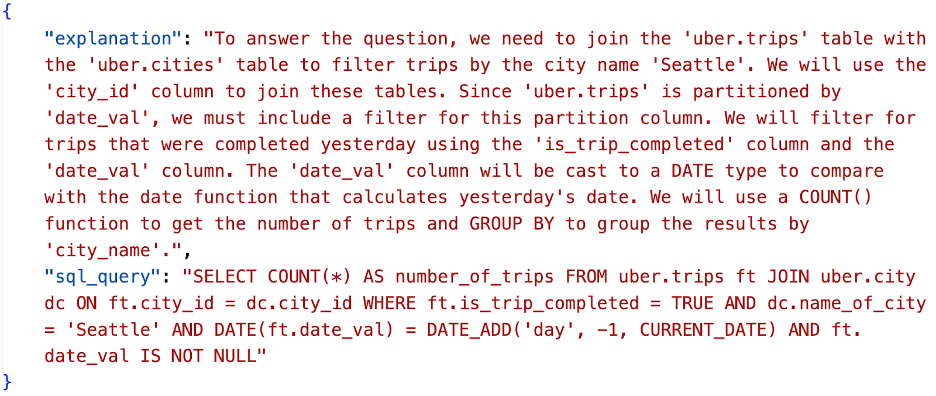
\includegraphics[width=10cm]{chapters/2/figures/query-gpt-output.png}
        \caption[Output of QueryGPT]{Output of QueryGPT  from~\cite{QueryGPT}}
        \label{fig:query-gpt-output}
    \end{figure}
        \subsubsection{Architecture Design}
        \begin{figure}[H]
            \centering
            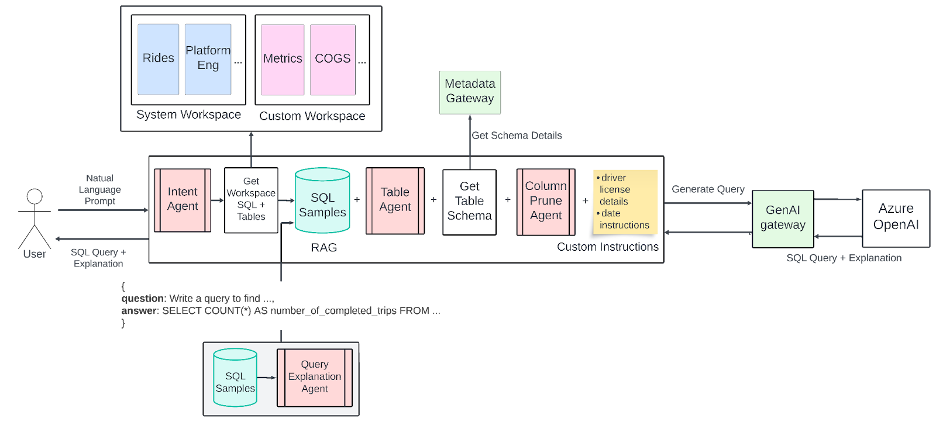
\includegraphics[width=10cm]{chapters/2/figures/query-gpt-architecture.png}
            \caption[QueryGPT Architecture Design]{QueryGPT Architecture Design  from~\cite{QueryGPT}}
            \label{fig:query-gpt-architecture}
        \end{figure}
        QueryGPT's architecture, as shown in Figure~\ref{fig:query-gpt-architecture}, is made up of several parts, but the four main ones are as follows:
\pagebreak
        \begin{itemize}
            \item  Workspaces

            Workspaces are collections of SQL samples and tables designed for specific business areas like Ads, Mobility, and Core Services. These aid in LLM concentration, increasing the precision of the inquiries that are produced. Workspaces are designed to narrow down the topic or domain that the user wants to focus on. By organizing SQL samples and tables into specific business areas (like Mobility, Ads, or IT), they help the system generate more relevant and accurate queries based on the user's needs. If none of the predefined "System Workspaces" fit, users can create their own "Custom Workspaces" to tailor the search further.
            \item  Intent Agent

            An Intent Agent is a system or tool that analyzes a user's question to determine its purpose or intent. In this case, it finds the business domain or workspace (like Mobility, Ads, or a custom workspace) the question belongs to. By doing so, it helps map the query to the relevant SQL samples and tables, ensuring more accurate and focused results. Essentially, it acts as a guide to direct the query to the right area of information.
            \item  Table Agent

            The purpose of the Table Agent is to guarantee that the appropriate tables are utilized when creating queries. Based on the user's query, it chooses the most relevant tables and shows them to the user for approval or modification. The user might choose to amend the current list and change the list of tables to be utilized, or they could click the "Looks Good" button in figure 2.8. This gives users greater control and improves the correctness of the results by ensuring that the appropriate tables are used for query generation.
            \item Column Prune Agent

            Table schemas can be made smaller by using the Column Prune Agent to eliminate unnecessary columns. As input to the LLM gets more focused and smaller, this helps improve query production by reducing token usage, reducing costs, and improving response time.
        \end{itemize}
        \begin{figure}[H]
            \centering
            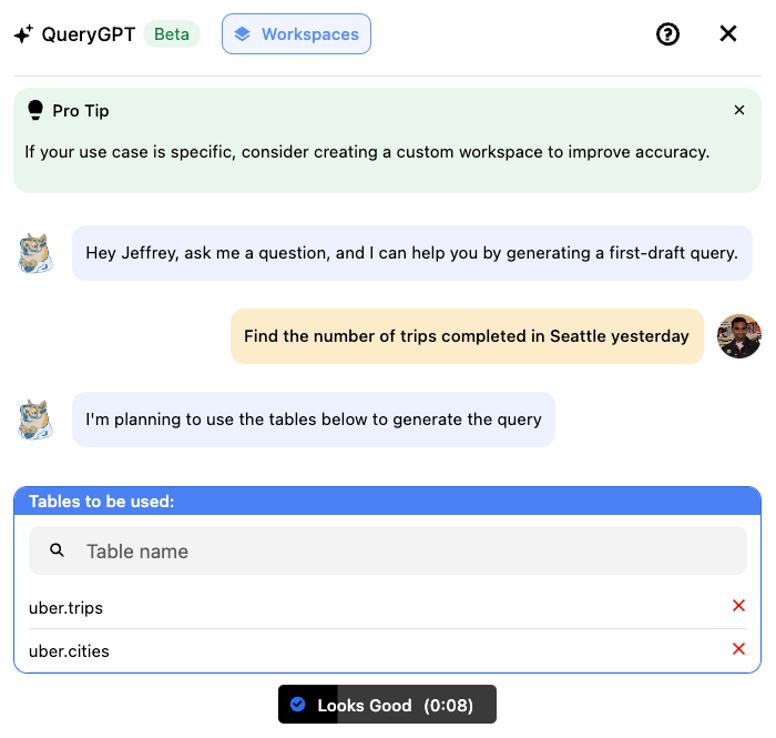
\includegraphics[width=8cm]{chapters/2/figures/query-gpt-ui.png}
            \caption[QueryGPT Interface]{QueryGPT Interface  from~\cite{QueryGPT}}
            \label{fig:query-gpt-interface}
        \end{figure}

        \subsubsection{Evaluation}
        The performance of QueryGPT was measured by two self-created evaluation processes called Vanilla and Decoupled. The Vanilla tests the entire process end-to-end and evaluates the results. On the other hand, Decoupled focuses on component-level evaluation by isolating steps. The "golden" question-to-SQL mappings in the examined data were hand-picked. Selecting actual queries from QueryGPT logs, confirming the right purpose, necessary schemas, and optimal SQL responses were all part of this process. The set consists of questions from a variety of business domains and datasets. In Figure~\ref{fig:query-gpt-metrics}, the evaluation metrics example is also displayed.
        To evaluate QueryGPT, the following metrics were tracked:
        \begin{itemize}
            \item  Intent Accuracy: Is the assigned intent correct for the question?
            \item  Table Overlap: Are the tables selected by Search + Table Agent correct? Scored between 0 and 1 based on how many required tables were identified.
            \item  Successful Run: Does the generated query execute successfully?
            \item  Run Has Output: Does the query return more than 0 records? (e.g., errors like incorrect filters can cause no output despite a successful run).
            \item  Query Similarity: How similar is the generated query to the golden SQL? An LLM assigns a similarity score (0 to 1) based on columns, joins, and functions.
        \end{itemize}
        \begin{figure}[H]
            \centering
            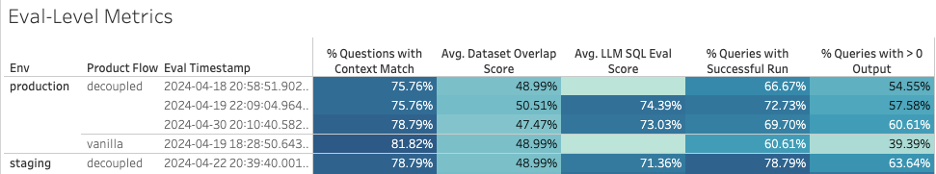
\includegraphics[width=10cm]{chapters/2/figures/query-gpt-metrics.png}
            \caption[Evaluation Metrics of QueryGPT]{Evaluation Metrics of QueryGPT  from~\cite{QueryGPT}}
            \label{fig:query-gpt-metrics}
        \end{figure}
    \subsection{Vanna.Ai}
    Vanna is an open-source Python framework designed for Retrieval-Augmented Generation (RAG) to facilitate SQL generation and related functionality. It uses Milvus as a vector database for efficient embedding similarity searches, ensuring accurate and relevant query handling.

    The framework includes two primary features: Train and Ask. The Train feature enables Vanna to learn and familiarize itself with metadata stored in Milvus, building a foundation for accurate query responses. The Ask feature serves as the main user interaction point, where users can ask SQL-related questions. Vanna utilizes the knowledge gained during training to generate precise SQL queries or responses.

    In addition to these features, Vanna incorporates a self-learning mechanism to enhance its ability to address future queries effectively. The framework also includes frontend integration, offering users a seamless and accessible interface for interaction.
    \cite{Vanna}

    Here are the highlighted advantages:
\pagebreak
    \begin{itemize}
        \item  Open-Source: The Vanna Python package and frontend integrations are open-source and can run on your infrastructure.
        \item  Security: Database contents are never sent to the LLM unless explicitly enabled; only schemas, documentation, and queries are stored.
        \item  Self-Learning: The model improves over time as training data is augmented through usage.
        \item  Database Support: Supports databases like Snowflake, BigQuery, Postgres, and more, with easy custom connector creation.
        \item  Flexible Frontend: Works with Jupyter Notebooks, Slackbot, web apps, Streamlit, or can integrate into your own web app.
    \end{itemize}
    \subsection{Summary}
    \begin{table}[H]
        \centering
        \caption{Comparison table between Query Assistance, SQLAI.ai, QueryGPT, and Vanna.AI}\label{tbl:compare}
        \includegraphics[width=15cm]{chapters/2/figures/table\_summary.png}
    \end{table}



    % \subsection{Algorithm I}
    % Add more subsections as you want.
    % \subsection{Algorithm II}
    %     Add more subsections as you want.
    %     \subsubsection{Step I}
    %         You can use subsection too!
    %     \subsubsection{Step II}
    %         This is the farthest level of subsection we permitted. (We support only 4th level)


    % \begin{table}[!h]
    % \caption{test table method1}\label{tbl:method1}
    %     \begin{tabular}{c|c|l|rr} \hline\hline
    %         Center & Center & left aligned & Right & Right aligned \\ \hline\hline
    %         Center & Center & left aligned & Right & Right aligned \\ \hline
    %         Center & Center & left aligned & Right & Right aligned \\
    %         Center & Center & left aligned & Right & Right aligned \\ \hline
    %         Center & Center & left aligned & Right & Right aligned \\ \hline\hline
    %     \end{tabular}
    % \end{table}

    % You can place any report elements and refer to it like Figure~\ref{tbl:method1}, \ref{fig:microservices-architecture}
    % The figure and table numbering will be run and updated automatically when you add/remove tables/figures from the document.

    % \begin{figure}[H]
    %     \centering
    %     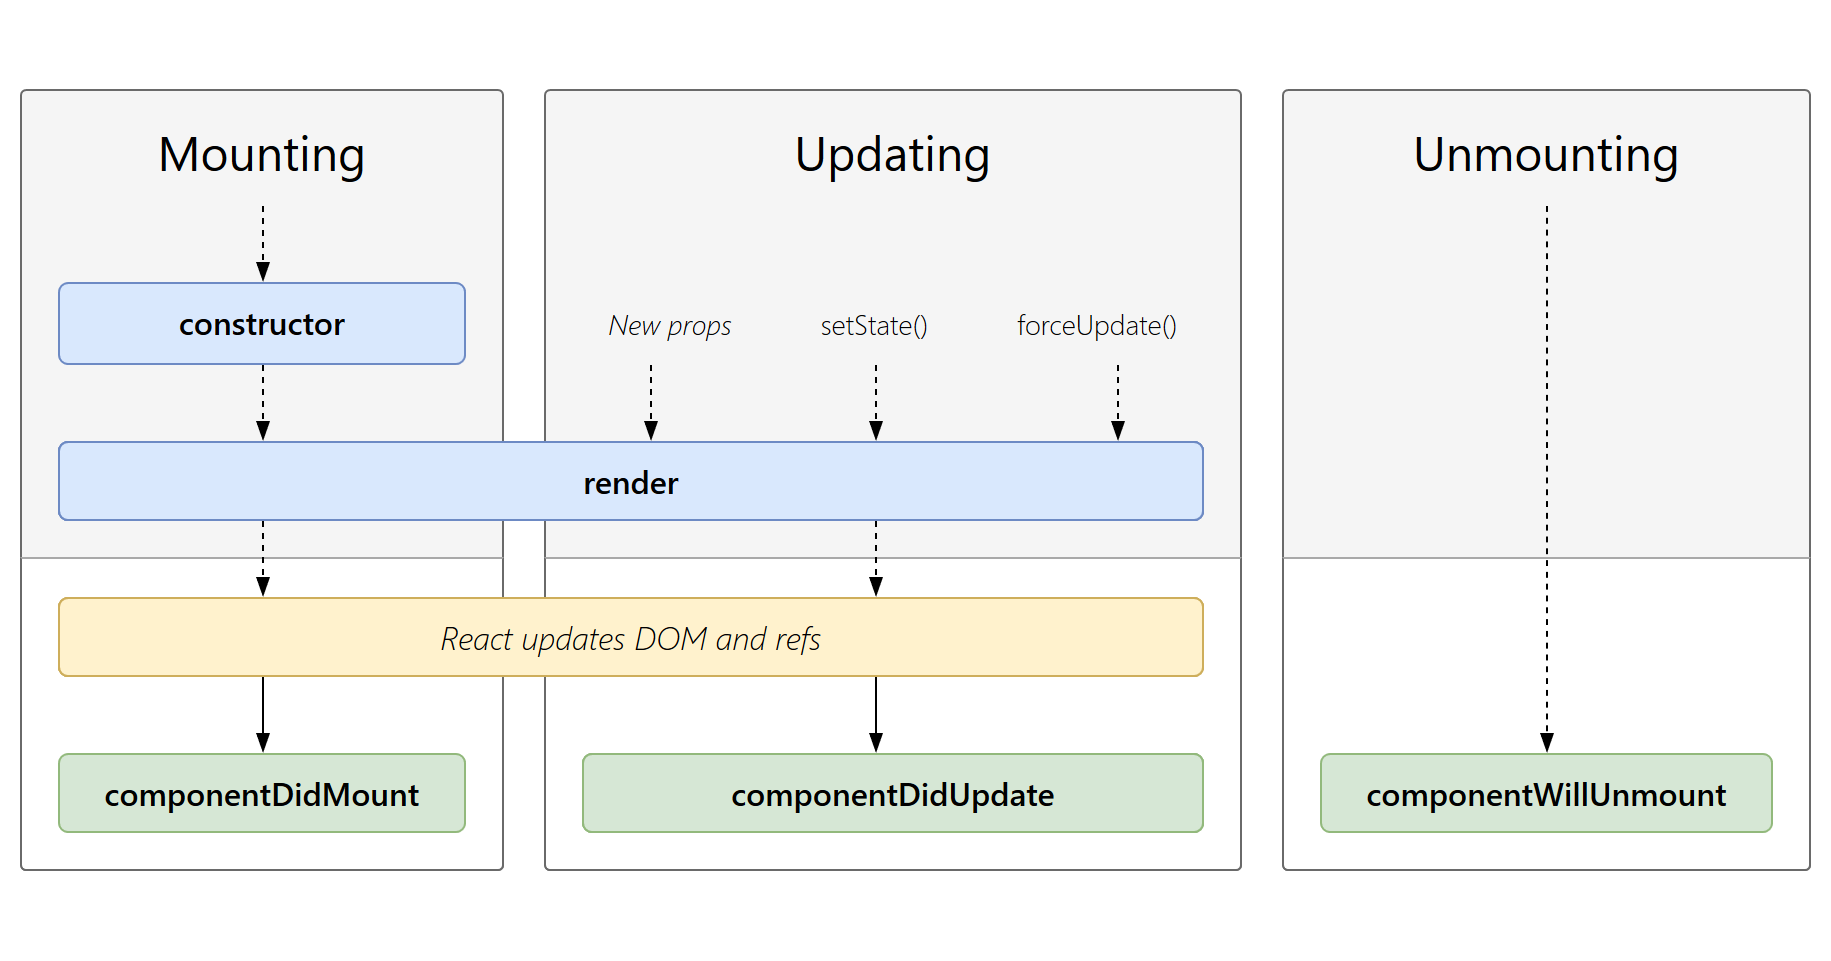
\includegraphics[width=7cm]{chapters/2/figures/react-lifecycle.png}
    %     \caption[Aspects of OOPs]{Aspects of OOPs from~\cite{bworld}}
    %     \label{fig:oop-concept}
    % \end{figure}




\pagebreak
